\begin{frame}
\setbeamercovered{invisible}
\frametitle{Outlook}




\begin{columns}[t]
\column{0.5\linewidth}
\textcolor{bellblue}{Dynamical instability}
\begin{figure}
\centering
\includegraphics[width=0.6\linewidth]{Figures/Instability.pdf}
\end{figure}
\bellRef{M. Abad et al.}{EPJD}{2015}
\vspace{0.4cm}

\textcolor{bellblue}{Finite temperature (four fluid model)}
\begin{figure}
\centering
\includegraphics[width=0.3\linewidth]{Figures/Thermal_Spinor.jpg}
\end{figure}
\bellRef{J. Armqitis et al.}{PRA}{2015}\\
\bellRef{K. L. Lee et al.}{PRA}{2016}

	
\column{0.5\linewidth}
\textcolor{bellblue}{Magnetic soliton}
\begin{figure}
\centering
\includegraphics[width=0.67\linewidth]{Figures/magneticsoliton.pdf}
\end{figure}

\bellRef{C. Qu et al.}{PRL}{2016}



\vspace{0.4cm}


\textcolor{bellblue}{Coherent coupling between spin components}\\
Many references and ideas...
\begin{figure}
\centering
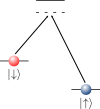
\includegraphics[width=0.4\linewidth]{Figures/Coherent_Coupling.pdf}
\end{figure}



\end{columns}


\end{frame}
